\documentclass{article}
\usepackage{fullpage}
\usepackage{graphicx}

\title{16.35 PSet \#3}
\author{Ryan Fish}
\date{\today}

\begin{document}
\maketitle

\section{Deliverables}
\subsection{Avoiding Deadlock}
\subsubsection{Plan}
Utilizing a directed graph image of our work thus far, reducing the number of cycles and preventing hold-and-wait where cycles could arise seemed the best form of deadlock prevention.  The Simulator class thread never needs to hold and wait (the clock may be incremented without other resources, and the position transmission to the server can be accomplished accessing only one vehicle at a time).  The GroundVehicle class thread also never executes a hold and wait, it is either in possession of the clock monitor, or it is in possession of its own monitor.  The VehicleController class threads are the ones at risk, for they can have the ability to acquire their own vehicle monitor and another vehicle monitor.  My method of preventing deadlock, even from a malicious implementation of VehicleController, will be to ensure VehicleControllers only have access to monitors they need (only GroundVehicles, the clock, and anything within their own class).  Additionally it is reasonable and within the specification to restrict VehicleControllers from hold and wait with GroundVehicles and the clock, since all controllers thus far only need access to the state of these individually. It is entirely possible to restrict them to sequential access to the necessary GroundVehicles and clock by privatizing these items (preventing monitor grabs) and making access to their state possible only through getter functions (preserving mutual exclusion and state access while removing the need for public object references).

Time Spent: 10 minutes

\subsubsection{Implementation}
My implementation of this restricted access to prevent wait-and-hold is held Simulator.  VehicleControllers only hold the hash of the GroundVehicle's they need reference to, and request state information to them through the mass store in Simulator.  No controllers used so far have needed any kind of hold-and-wait for operation, so no additional implementation is required.

Time Spent: 20 minutes

\subsection{addGroundVehicle tests}
Since we now have extended Thread with Simulator, it seems likely we may start sharing sets of vehicles.  I have modified and tested \verb|addGroundVehicle| so that it is thread safe, so even highly concurrent vehicle adding is safe.  My code still makes the assumption that the simulation will only be triggered once all vehicles are added.

Time Spent: 20 minutes

\subsection{LeaderController}
\begin{center}
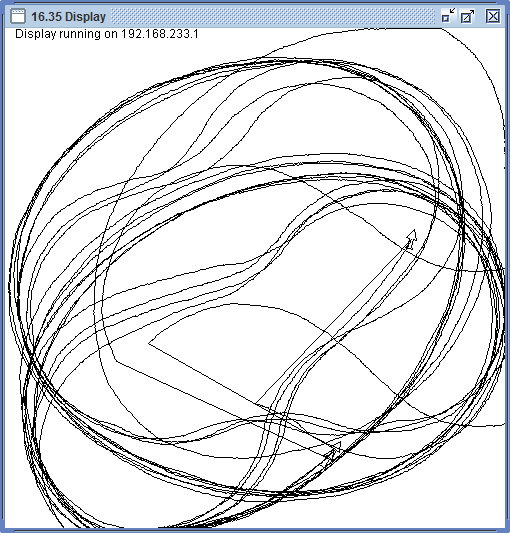
\includegraphics[width=0.7\linewidth]{leader}
\end{center}

\subsection{LeaderController code and various fixes}
Time Spent: 2 hours



\section{Predeliverables}
\subsection{Test Case Rationale}

My addVehicle method simply adds a reference to the vehicle to a list of all vehicles so that it's state can be gathered later by the Simulator.  The important stuff happens upon construction of the vehicle and controller, where it adds itself to the set of threads that must run in lockstep with the time incrementation.  Since the predeliverable implementation is just wait for time, set speeds and update positions, I just check to make sure that adding a vehicle or controller increments the count, that getting the time decrements the count, and incrementing the time resets the count.

\subsection{No Noise, 5 Vehicles}

\begin{center}
	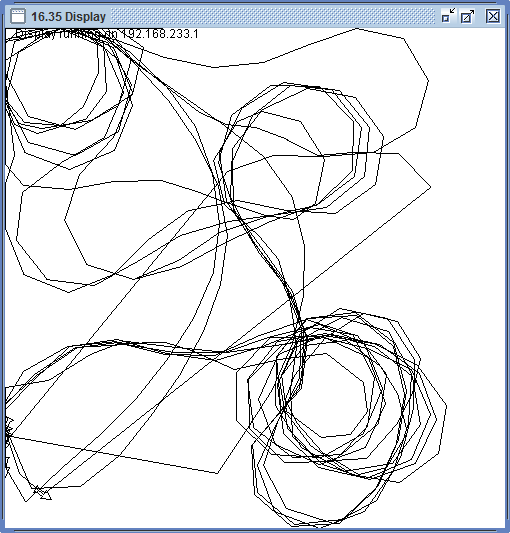
\includegraphics[width=0.7\linewidth]{5nonoise}
\end{center}

\subsection{Noise, 5 Vehicles}

\begin{center}
	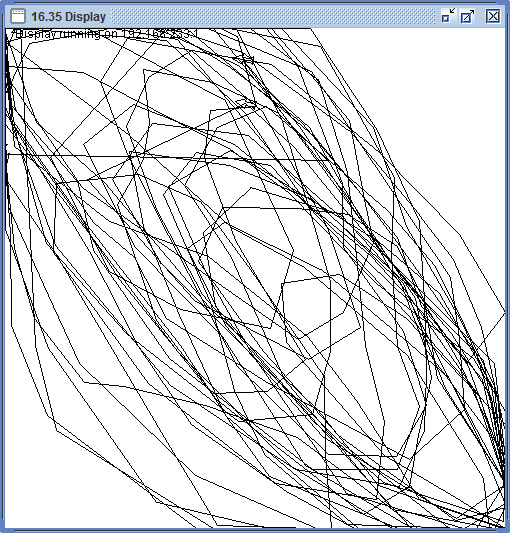
\includegraphics[width=0.7\linewidth]{5noise}
\end{center}


\subsection{4 Conditions of Deadlock and You}

\begin{enumerate}
	\item[MutEx] We need to prevent reads occurring concurrently with writes to vehicle state.
	\item[Hold and Wait] In particular, LeadingController may grab its own state and wait for a lock on the state of a vehicle it is leading.
	\item[No Preemption]  Without modification, the default synchronization system of Java does not allow for preemption in acquisition of resources.
	\item[Circular Wait]  A Leading Controller may wait on acquisition of the state of a Following controller, who is waiting to acquire the state of the same LeadingController.
\end{enumerate}
\subsection{Proposal for Avoiding Deadlock} 

The best way to attack deadlock in this scenario would be to attack circular wait.  I will build an object to manage monitor acquisition that will assign a monotonically increasing index to object classes able to be locked, and prevent acquisition of an index lower than the highest one held.  It will trigger a release of any objects held with higher indexes.


\end{document}
